\documentclass{article}
\usepackage[utf8]{inputenc}
\usepackage{graphicx}

\begin{document}
\title{Exercise 1 of the Computer Vision course at the
  University of Helsinki in May 2018}

\author{\emph{Konsta Kutvonen}}
\maketitle


\newpage
\section{Hands on exercises}

\subsection{Original, noisy and filtered images}

\newcommand{\aaa}[3]{%
  \fbox{\includegraphics[height=30mm,draft]{#1}} \quad
  \fbox{\includegraphics[height=30mm,draft]{#2}} \quad
  \fbox{\includegraphics[height=30mm,draft]{#3}} \par}

\newcommand{\bbb}[3]{%
  \medskip\noindent\aaa{#1}{#1-#2}{#1-#3}}

\setlength{\fboxsep}{0pt}%

pattern low pass


\fbox{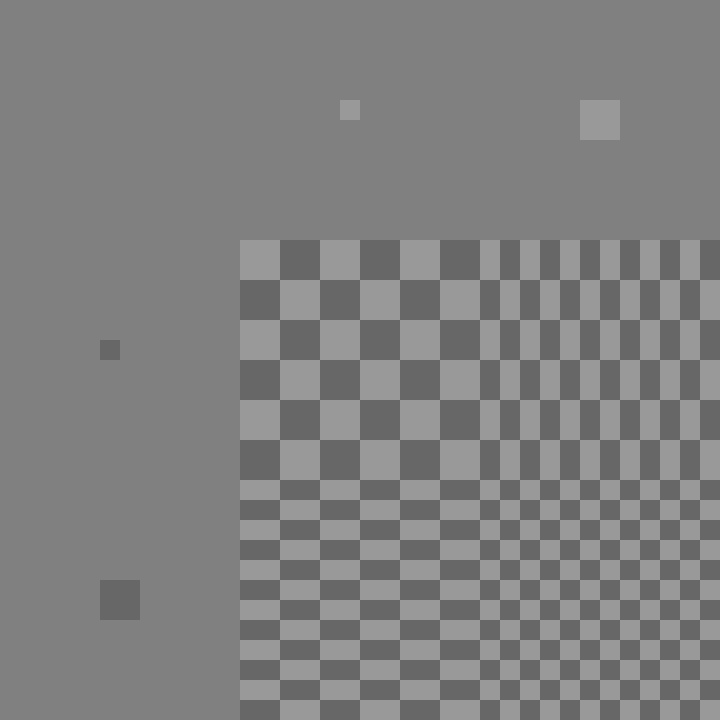
\includegraphics[height=30mm]{p}}
\fbox{
\includegraphics[height=30mm]{pl3}}
\fbox{
\includegraphics[height=30mm]{pl5}}

\fbox{
\includegraphics[height=30mm]{pg05}}
\fbox{
\includegraphics[height=30mm]{pl3g05}}
\fbox{
\includegraphics[height=30mm]{pl5g05}}


\fbox{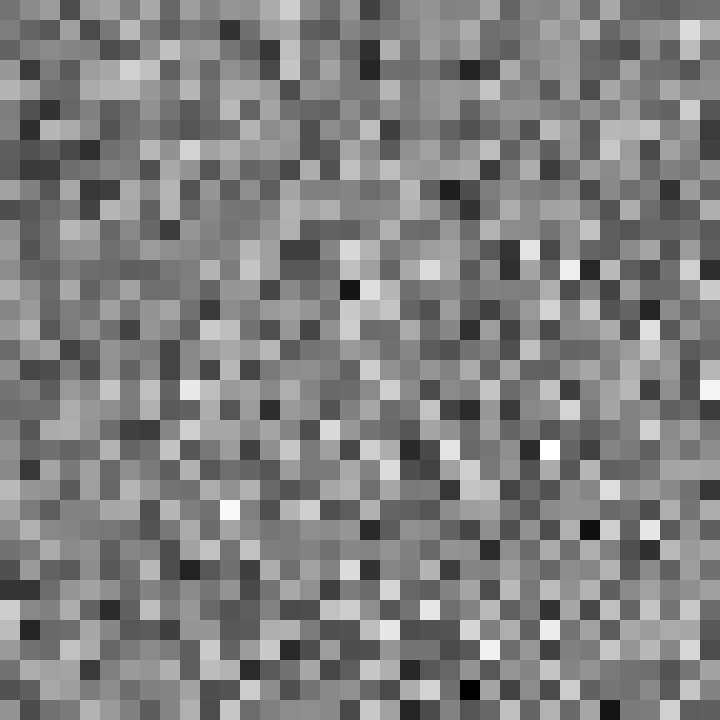
\includegraphics[height=30mm]{pg15}}
\fbox{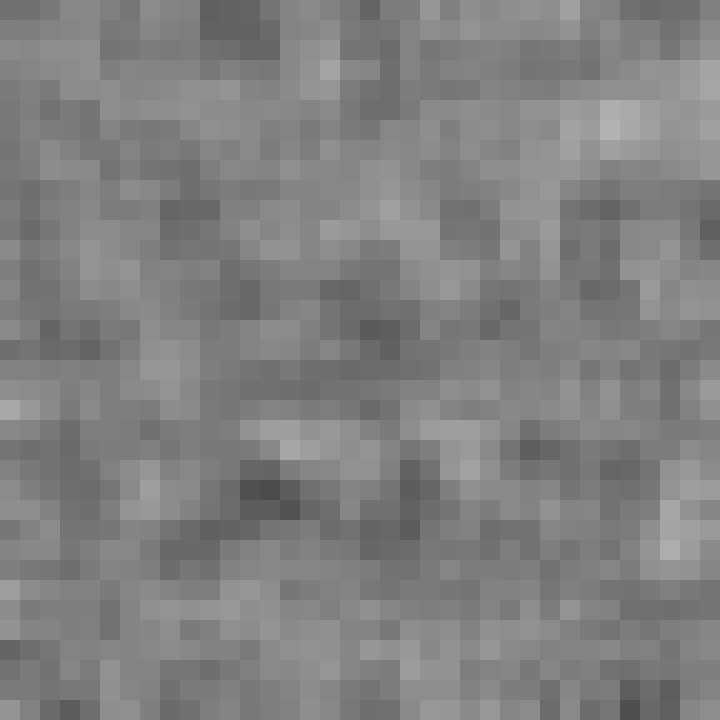
\includegraphics[height=30mm]{pl3g15}}
\fbox{
\includegraphics[height=30mm]{pl5g15}}


\fbox{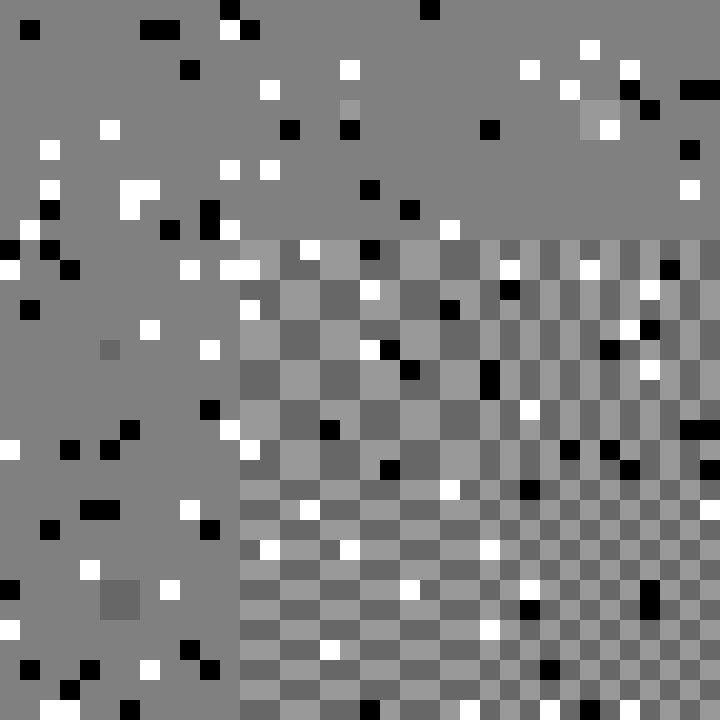
\includegraphics[height=30mm]{psp1}}
\fbox{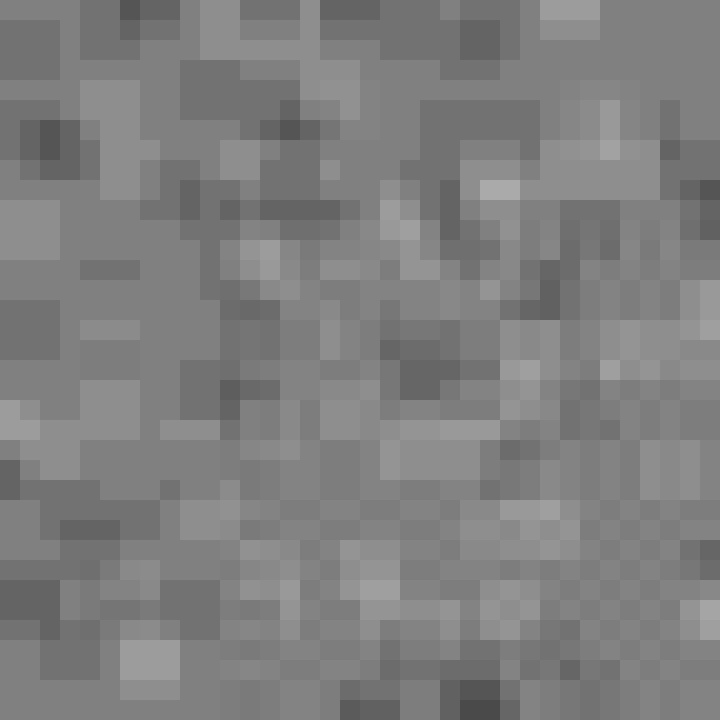
\includegraphics[height=30mm]{pl3sp1}}
\fbox{
\includegraphics[height=30mm]{pl5sp1}}


\fbox{
\includegraphics[height=30mm]{psp5}}
\fbox{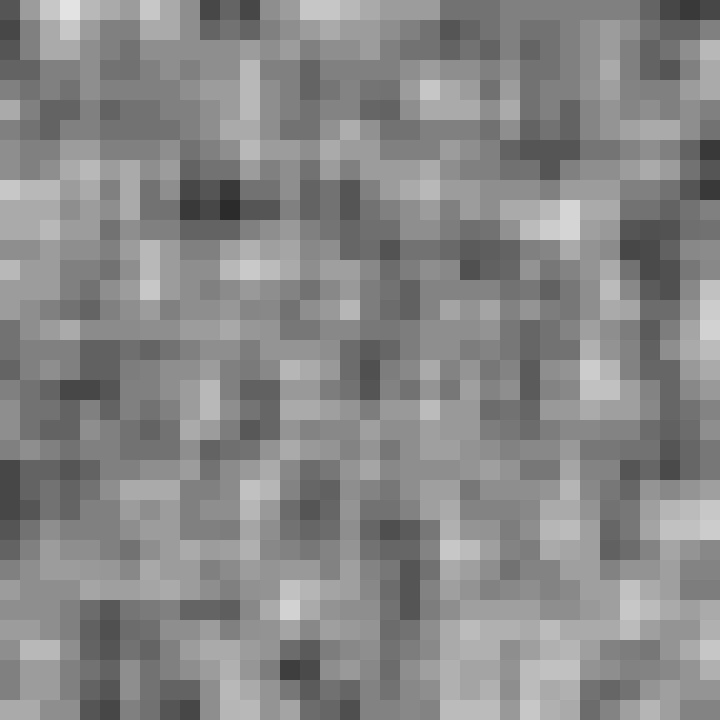
\includegraphics[height=30mm]{pl3sp5}}
\fbox{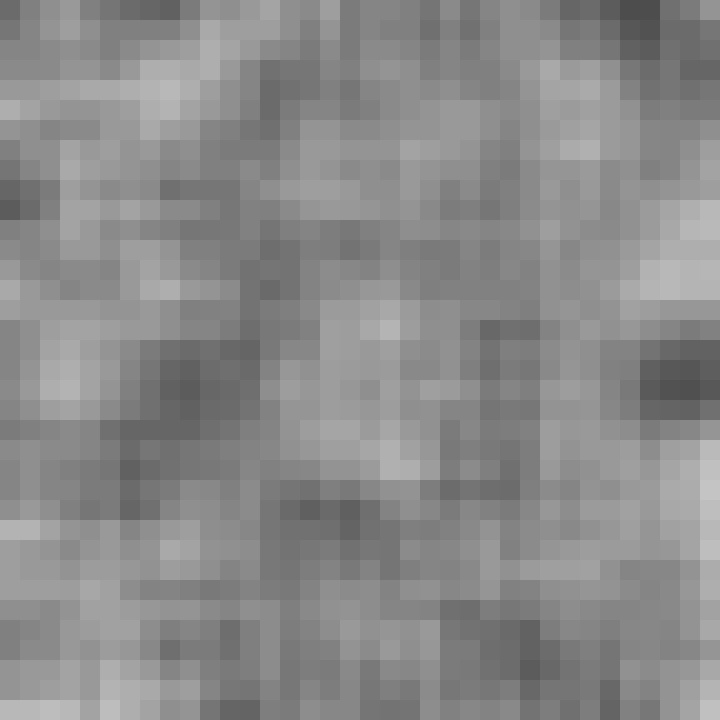
\includegraphics[height=30mm]{pl5sp5}}

\pagebreak


messi low pass


\fbox{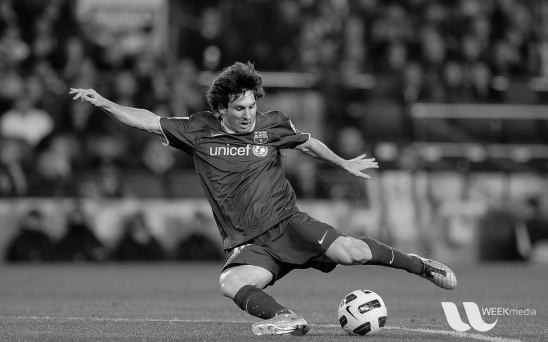
\includegraphics[height=30mm]{m}}
\fbox{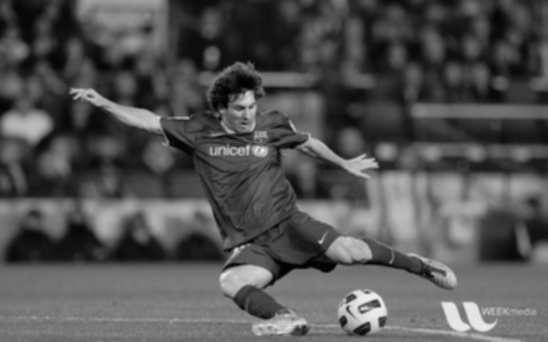
\includegraphics[height=30mm]{ml3}}
\fbox{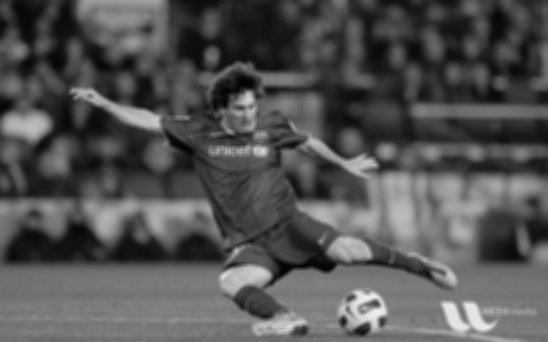
\includegraphics[height=30mm]{ml5}}

\fbox{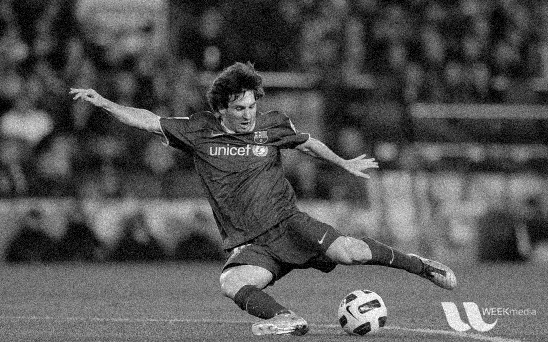
\includegraphics[height=30mm]{mg05}}
\fbox{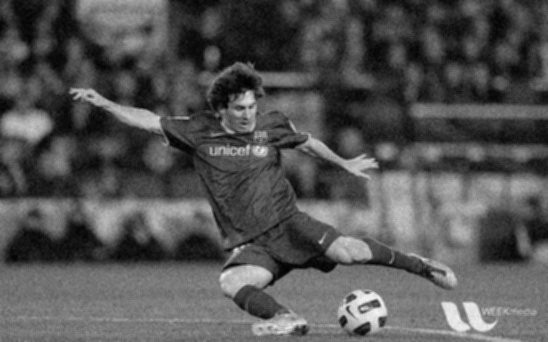
\includegraphics[height=30mm]{ml3g05}}
\fbox{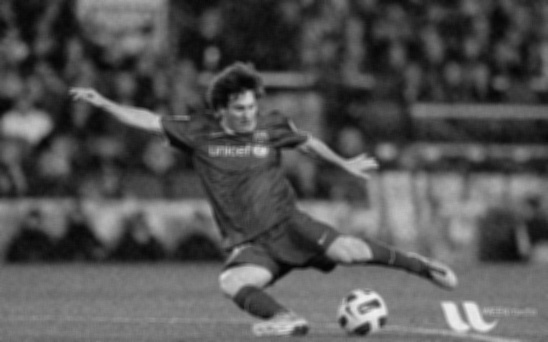
\includegraphics[height=30mm]{ml5g05}}


\fbox{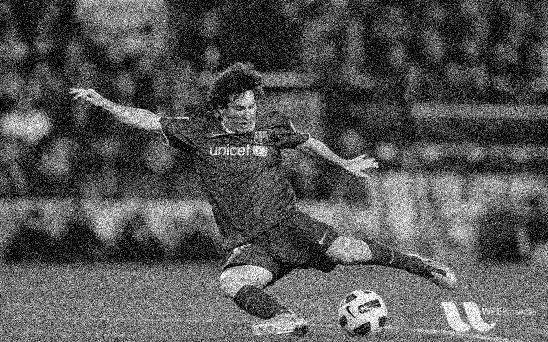
\includegraphics[height=30mm]{mg15}}
\fbox{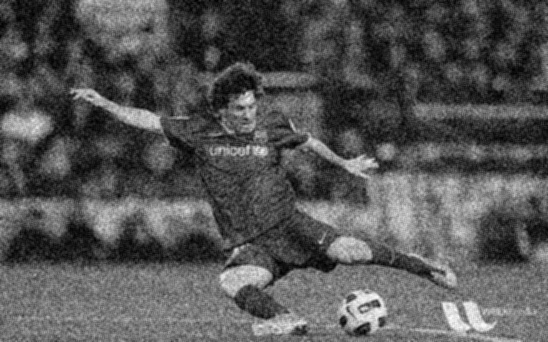
\includegraphics[height=30mm]{ml3g15}}
\fbox{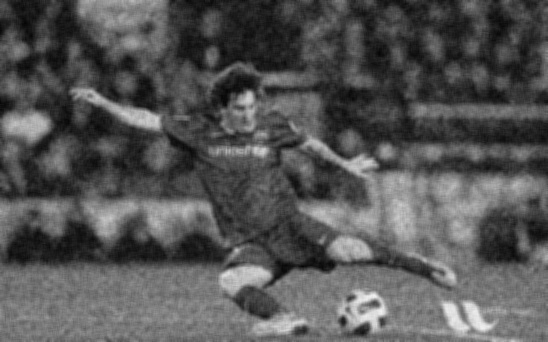
\includegraphics[height=30mm]{ml5g15}}


\fbox{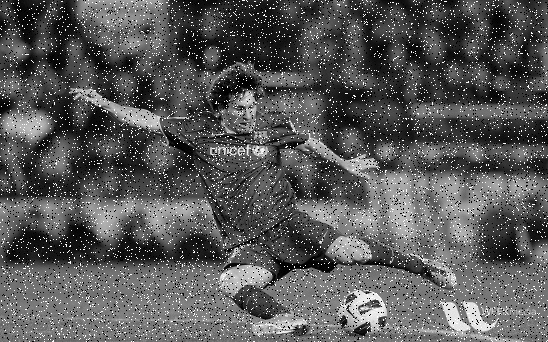
\includegraphics[height=30mm]{msp1}}
\fbox{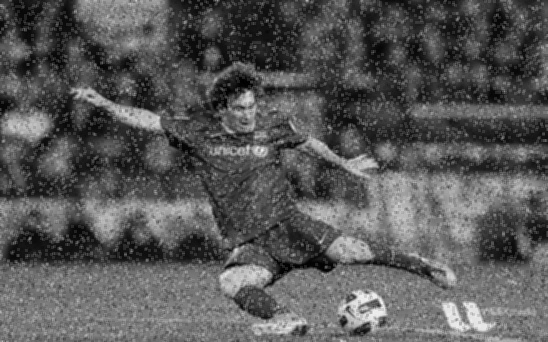
\includegraphics[height=30mm]{ml3sp1}}
\fbox{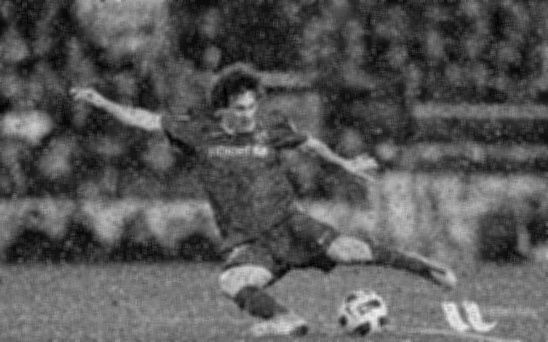
\includegraphics[height=30mm]{ml5sp1}}


\fbox{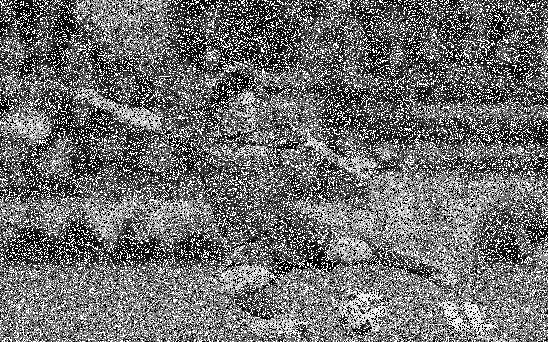
\includegraphics[height=30mm]{msp5}}
\fbox{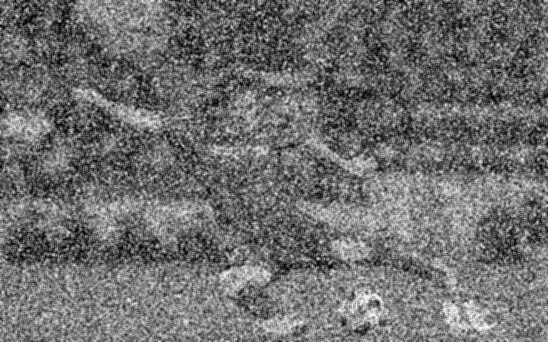
\includegraphics[height=30mm]{ml3sp5}}
\fbox{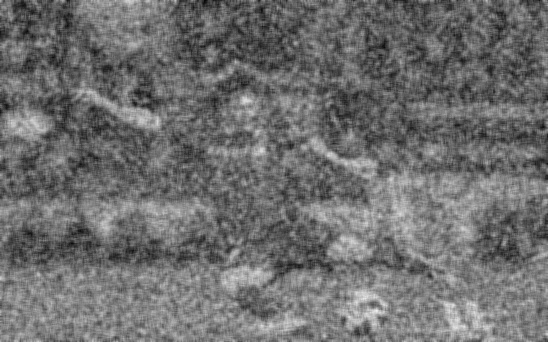
\includegraphics[height=30mm]{ml5sp5}}

\pagebreak

pattern median

\fbox{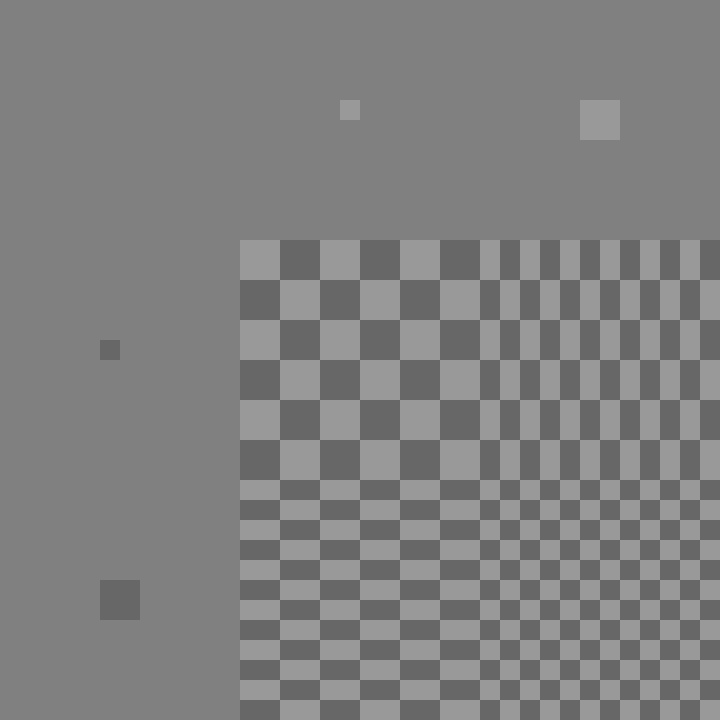
\includegraphics[height=30mm]{p}}
\fbox{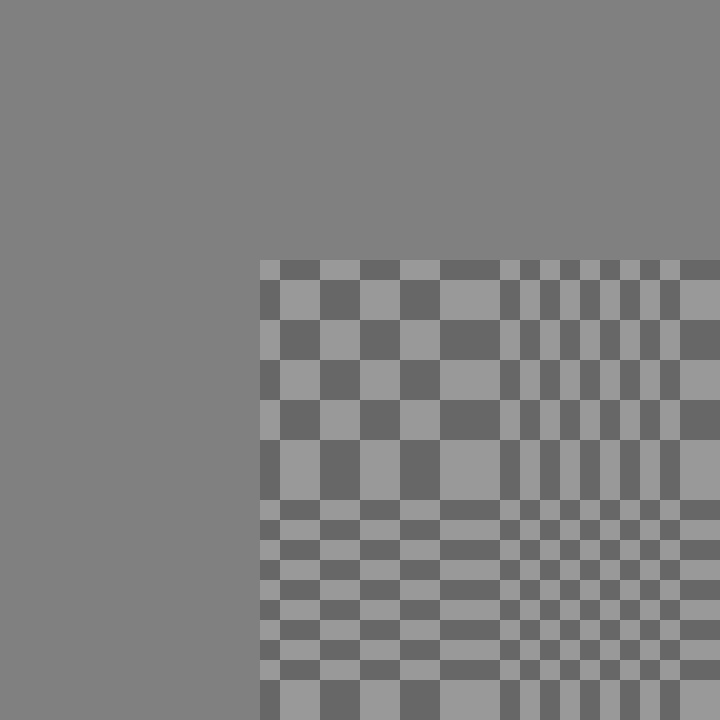
\includegraphics[height=30mm]{pm3}}
\fbox{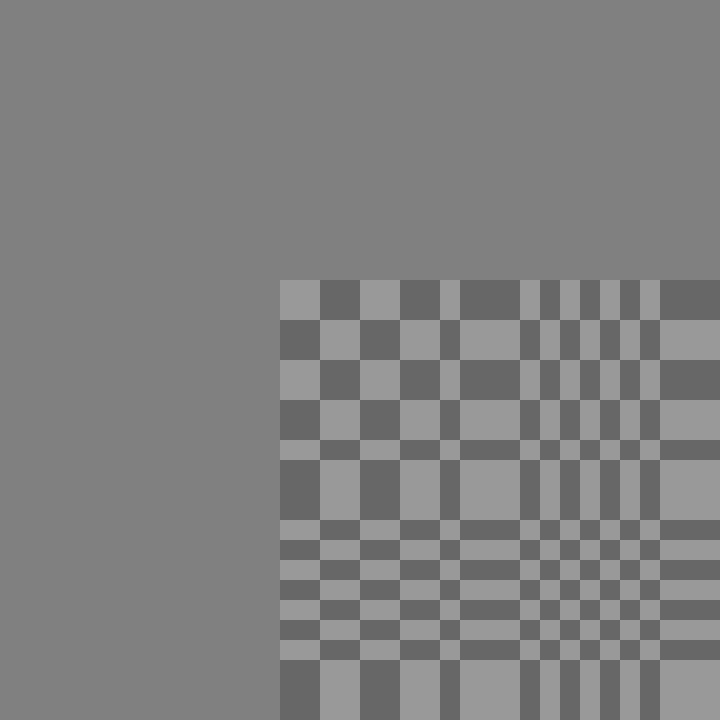
\includegraphics[height=30mm]{pm5}}

\fbox{
\includegraphics[height=30mm]{pg05}}
\fbox{
\includegraphics[height=30mm]{pm3g05}}
\fbox{
\includegraphics[height=30mm]{pm5g05}}


\fbox{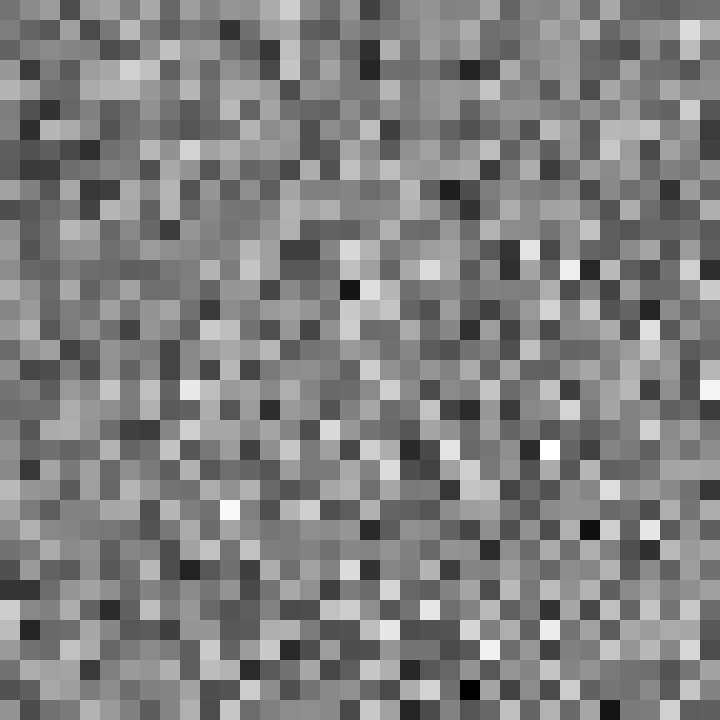
\includegraphics[height=30mm]{pg15}}
\fbox{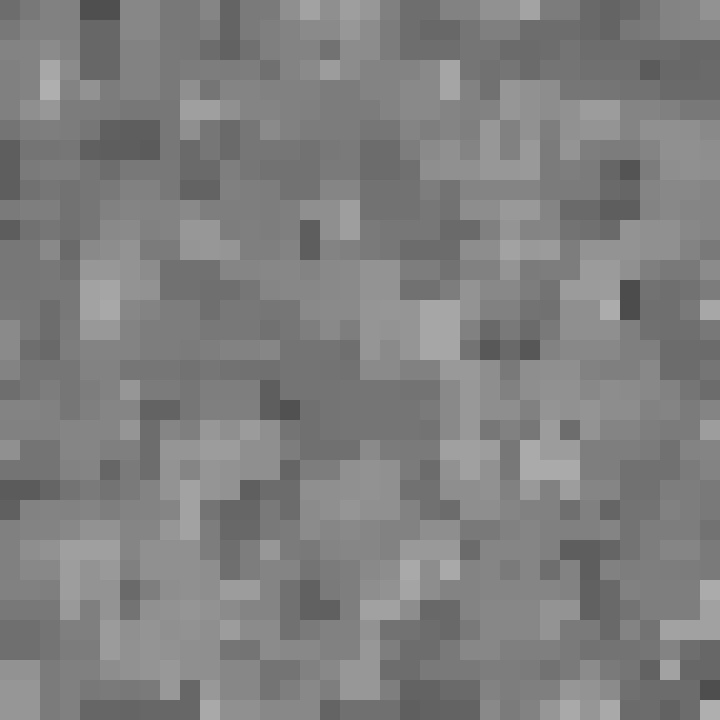
\includegraphics[height=30mm]{pm3g15}}
\fbox{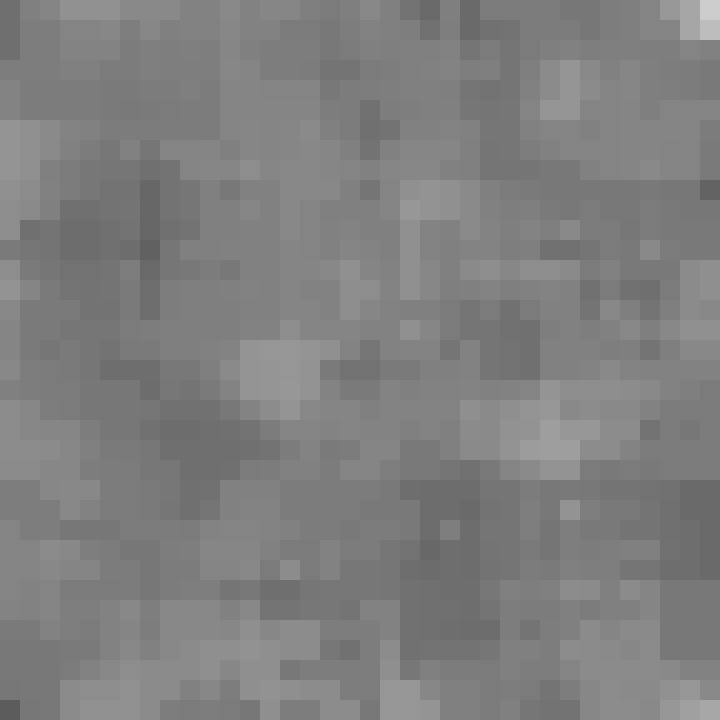
\includegraphics[height=30mm]{pm5g15}}


\fbox{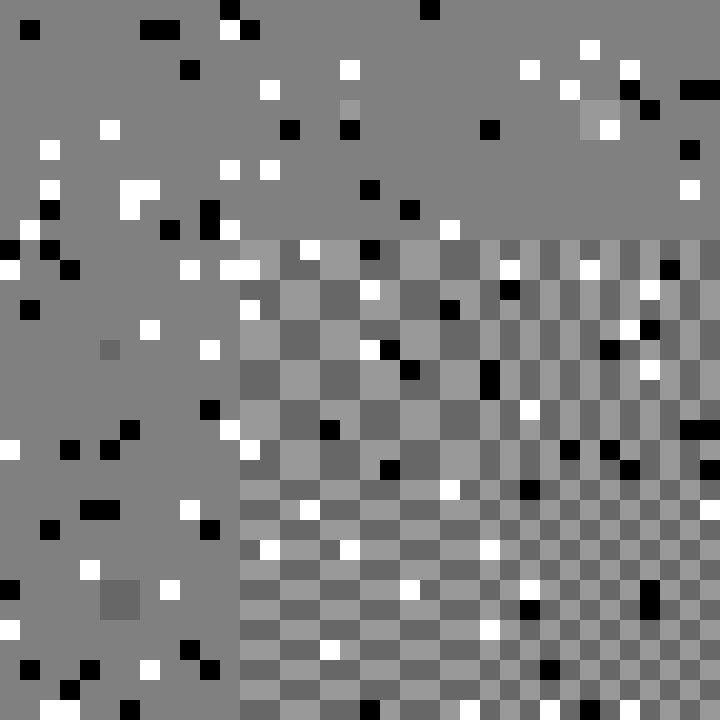
\includegraphics[height=30mm]{psp1}}
\fbox{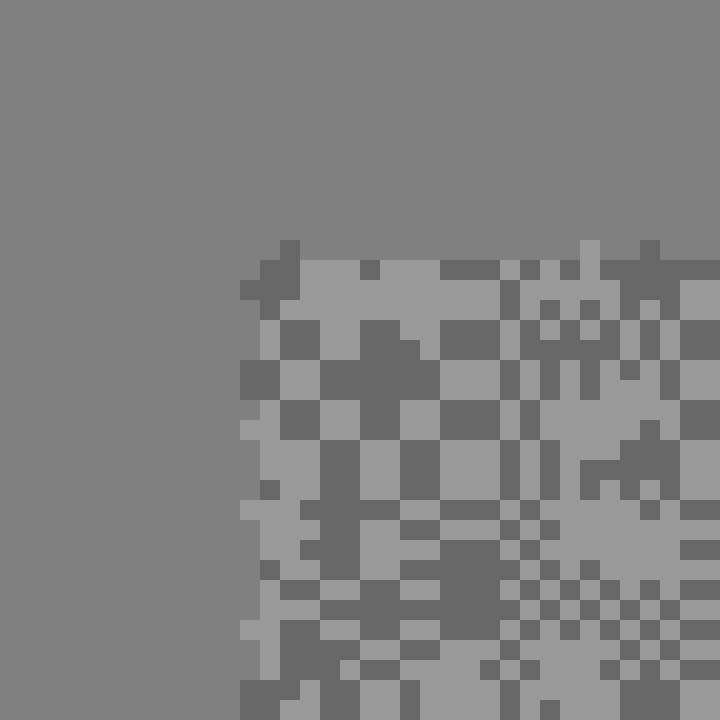
\includegraphics[height=30mm]{pm3sp1}}
\fbox{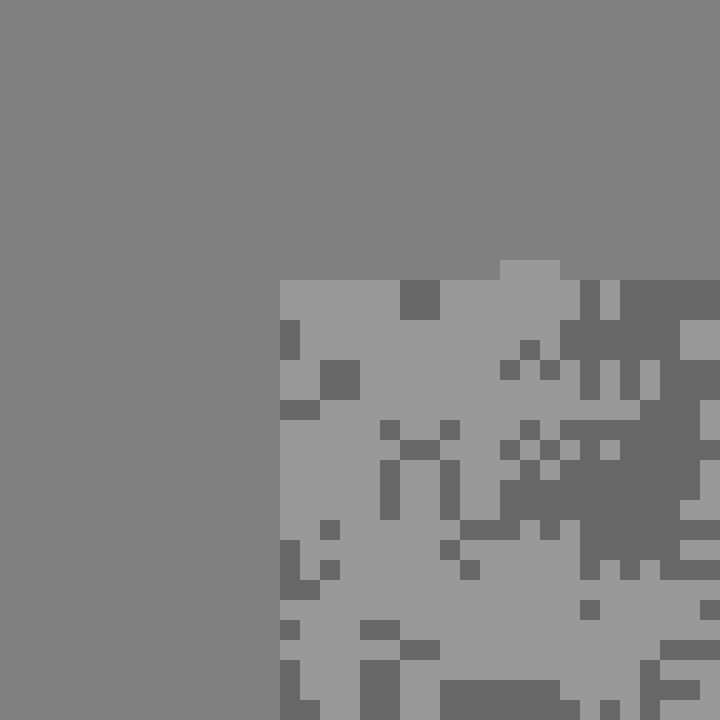
\includegraphics[height=30mm]{pm5sp1}}


\fbox{
\includegraphics[height=30mm]{psp5}}
\fbox{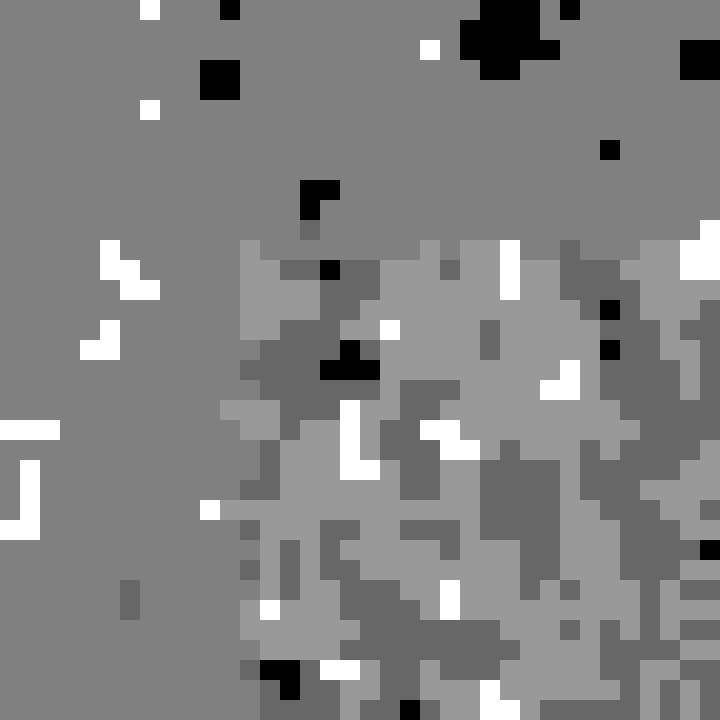
\includegraphics[height=30mm]{pm3sp5}}
\fbox{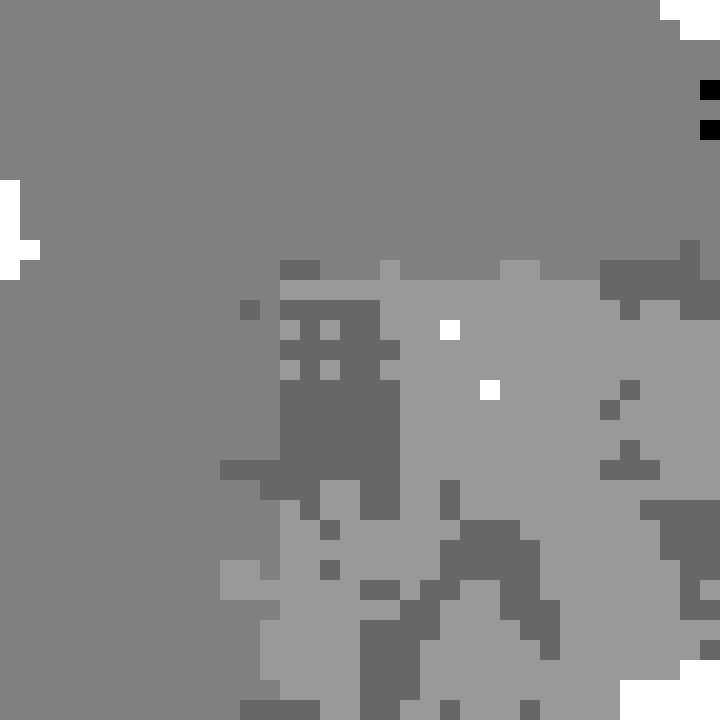
\includegraphics[height=30mm]{pm5sp5}}

\pagebreak

messi median

\fbox{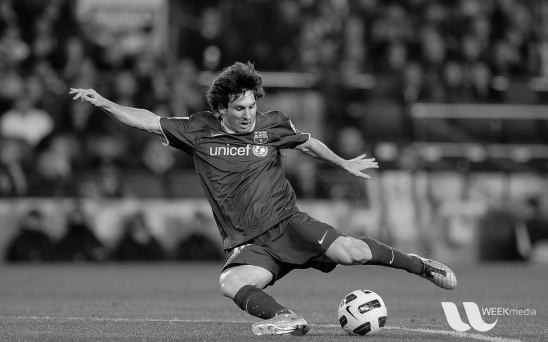
\includegraphics[height=30mm]{m}}
\fbox{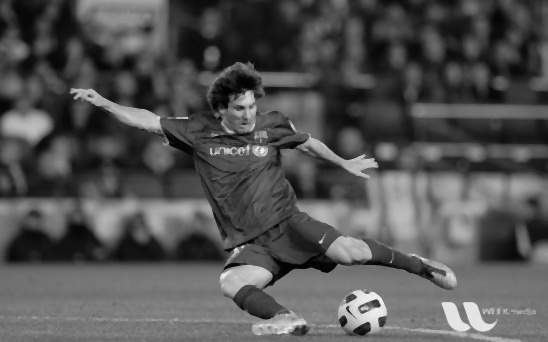
\includegraphics[height=30mm]{mm3}}
\fbox{\includegraphics[height=30mm]{mm5}}

\fbox{\includegraphics[height=30mm]{mg05}}
\fbox{\includegraphics[height=30mm]{mm3g05}}
\fbox{\includegraphics[height=30mm]{mm5g05}}


\fbox{\includegraphics[height=30mm]{mg15}}
\fbox{\includegraphics[height=30mm]{mm3g15}}
\fbox{\includegraphics[height=30mm]{mm5g15}}


\fbox{\includegraphics[height=30mm]{msp1}}
\fbox{\includegraphics[height=30mm]{mm3sp1}}
\fbox{\includegraphics[height=30mm]{mm5sp1}}


\fbox{\includegraphics[height=30mm]{msp5}}
\fbox{\includegraphics[height=30mm]{mm3sp5}}
\fbox{\includegraphics[height=30mm]{mm5sp5}}

\pagebreak

pattern high pass

\fbox{\includegraphics[height=30mm]{p}}
\fbox{\includegraphics[height=30mm]{ph3}}
\fbox{\includegraphics[height=30mm]{ph5}}

\fbox{\includegraphics[height=30mm]{pg05}}
\fbox{\includegraphics[height=30mm]{ph3g05}}
\fbox{\includegraphics[height=30mm]{ph5g05}}


\fbox{\includegraphics[height=30mm]{pg15}}
\fbox{\includegraphics[height=30mm]{ph3g15}}
\fbox{\includegraphics[height=30mm]{ph5g15}}


\fbox{\includegraphics[height=30mm]{psp1}}
\fbox{\includegraphics[height=30mm]{ph3sp1}}
\fbox{\includegraphics[height=30mm]{ph5sp1}}


\fbox{\includegraphics[height=30mm]{psp5}}
\fbox{\includegraphics[height=30mm]{ph3sp5}}
\fbox{\includegraphics[height=30mm]{ph5sp5}}

\pagebreak

messi high pass 

\fbox{\includegraphics[height=30mm]{m}}
\fbox{\includegraphics[height=30mm]{mh3}}
\fbox{\includegraphics[height=30mm]{mh5}}

\fbox{\includegraphics[height=30mm]{mg05}}
\fbox{\includegraphics[height=30mm]{mh3g05}}
\fbox{\includegraphics[height=30mm]{mh5g05}}


\fbox{\includegraphics[height=30mm]{mg15}}
\fbox{\includegraphics[height=30mm]{mh3g15}}
\fbox{\includegraphics[height=30mm]{mh5g15}}


\fbox{\includegraphics[height=30mm]{msp1}}
\fbox{\includegraphics[height=30mm]{mh3sp1}}
\fbox{\includegraphics[height=30mm]{mh5sp1}}


\fbox{\includegraphics[height=30mm]{msp5}}
\fbox{\includegraphics[height=30mm]{mh3sp5}}
\fbox{\includegraphics[height=30mm]{mh5sp5}}

\pagebreak
\subsection{Questions}
a) PBM is easy to handle even with just a text editor. TIFF is a lossless image format.

b) There is one just grey square, one grey square with a small lighter grey square inside it, one grey square with a similar lighter grey square but one that is larger, two similar squares but with dark squares inside. The remaining four squares are chessboard patterns, two of them properly scaled. The bottom-right checkerboard pattern has the highest possible frequency as every other pixel has a different. The other properly scaled chessboard has half the frequency of that. Then there are ones that have vertically maximum frequency and horizontally half that frequency and the other vice versa.
\pagebreak

\subsection{Pre and post normalization histograms}

\fbox{\includegraphics[height=45mm]{prenormal}}
\fbox{\includegraphics[height=45mm]{postnormal}}

\subsection{Effects of filterings}

The high pass filter leaves the image with just the outlines of the shapes in it. This can clearly be seen in the Messi images. Even in the heavy pepper and salt image you still can kind of tell the outline of Messi. Similar thing can be seen in the first pattern image, the others kind of show the same signs but especially the heavily noisy images are nearly uncomprehensible.

The low pass filter blurs the images and thus it removes some of the noise. This blurring effect can be especially seen on the pattern images, and they all turn into completely uncomprehensible after the low pass filter if there is any noise. The blur effect can also be easily seen on the Messi images and it does remove the normal noise, but it does not really work against the pepper and salt.

The median actually is able to preserve some kind of structure from the pattern images even if they are noisy. It does quite well with both the noises, but especially in the pepper and salt case it outshines the low pass filter. It does lose more details from the image though, this is apparent in Messi's face. Also due to the large amount of noise in one area, it can leave the median being 0 or 1 in some cases so it doesn't get rid of all the noise. This could be improved with larger window, but it would also cause more loss of quality.

\subsection{The code}
\begin{verbatim}
#! /usr/bin/env python3

import cv2
import numpy as np
from matplotlib import pyplot as plt
import math


def random_gauss(A, r):
    return clip(A + np.random.normal(0, r, A.shape))


def clip(i):
    return np.clip(i, 0, 1)


def random_saltpepper(A, r):
    prob = r / 2
    peppers = np.random.binomial(1, r/2, size=A.shape)
    A = clip(A - peppers)
    salts = np.random.binomial(1, r/2, size=A.shape)
    A = clip(A + salts)
    return clip(A)


def lowpass(A, n):
    filter = 1/(n*n)
    newA = np.array(A, copy=True)
    pad = (n - 1) // 2
    A = np.pad(A, pad, 'edge')
    x, y = A.shape
    for a in range (0, x - n + 1):
        for b in range(0, y - n + 1 ):
            newA[a, b] = np.sum(filter * (submatrix(A, a, b, n)))
    return clip(newA)


def highpass(A, n):
    filter = np.full((n, n), -1/(n*n - 1))
    filter[((n)//2, (n)//2)] = 1
    newA = np.array(A, copy=True)
    pad = (n - 1) // 2
    A = np.pad(A, pad, 'edge')
    x, y = A.shape
    for a in range (0, x - n//2):
        for b in range(0, y - n//2):
            sm = submatrix(A, a, b, n)
            if sm.shape == filter.shape:
                newA[(a, b)] = np.sum(np.multiply(filter, (submatrix(A, a, b, n))))
    return (newA)


def median(A, n):
    filter = np.full((n, n), -1/(n*n - 1))
    filter[((n)//2, (n)//2)] = 1
    newA = np.array(A, copy=True)
    pad = (n - 1) // 2
    A = np.pad(A, pad, 'edge')
    x, y = A.shape
    for a in range (0, x):
        for b in range(0, y):
            sm = submatrix(A, a, b, n)
            if sm.shape == filter.shape:
                newA[(a, b)] = np.median(submatrix(A, a, b, n))
    return clip(newA)

        
def submatrix(matrix, startRow, startCol, size):
    return matrix[startRow:startRow+size,startCol:startCol+size]


print('Reading images')

p = cv2.imread('pattern.pbm',     cv2.IMREAD_GRAYSCALE)/255
m = cv2.imread('messi-gray.tiff', cv2.IMREAD_GRAYSCALE)/255

img = cv2.imread('messi-gray.tiff', cv2.IMREAD_GRAYSCALE)
equ = cv2.equalizeHist(img)

hist, bins = np.histogram(equ.flatten(),256,[0,256])
plt.hist((equ).flatten(),256,[0,256], color = 'r')
plt.xlim([0,256])
plt.legend(('histogram'), loc = 'upper left')
plt.savefig('postnormal.png')
plt.show()

hist, bins = np.histogram((m * 255).flatten(),256,[0,256])
cdf = hist.cumsum()
plt.hist((m* 255).flatten(),256,[0,256], color = 'r')
plt.xlim([0,256])
plt.legend(('histogram'), loc = 'upper left')
plt.savefig('prenormal.png')
\end{verbatim}

Also some really exciting image creation and saving, which are pasted at the very end of this document.

\subsection{Time}
This took about 7 hours
\newpage
\section{Strawberries, strawberries, strawberries}
\subsection{Plot of pixels by radius}



\fbox{\includegraphics[height=85mm]{redgreen}}

The used RGB points were (190, 40, 30) for red, (120, 150, 40) for green.

\newpage
\subsection{Binary masks}
I took the binary masks with the intensity values of 40, 50, 60 and 70 for both red and green masks. They are here in the same order.


\subsection{Red binary masks}
\fbox{\includegraphics[height=70mm]{red-40}}
\fbox{\includegraphics[height=70mm]{red-50}}
\fbox{\includegraphics[height=70mm]{red-60}}
\fbox{\includegraphics[height=70mm]{red-70}}
\newpage
\subsection{Green binary masks}
\fbox{\includegraphics[height=70mm]{green1-40}}
\fbox{\includegraphics[height=70mm]{green1-50}}
\fbox{\includegraphics[height=70mm]{green1-60}}
\fbox{\includegraphics[height=70mm]{green1-70}}
\subsection{Combined mask}
\fbox{\includegraphics[height=120mm]{combine}}
\subsection{Decent threshold}
As can be observed from the images, the intensity at 70 seemed to work quite well with both of the colors that were used in creating these images. Below 70 there were some parts of the desired colors that were not included and at 70 and above other parts of the picture started to get included in the mask. From the graph these points are not really visible. Red seems to climb quite linearly until radius 160 and green spikes soon after 100. These are the points where large amounts of the rest of the image gets included, but before then also some undesired parts get to become part of the mask so they are not necessarily the best intensities to use.
\newpage
\subsection{Code}
\begin{verbatim}
str = cv2.imread('strawberries.tiff')

def removecolor(A, R, G, B, d):
    accepted = 0
    AA = np.array(A, copy=True)
    for i in range (len(A)):
        row = A[i]
        for j in range (len(row)):
            (eb, eg, er) = row[j]
            dist = (er - R)**2 + (eg - G)**2 + (eb - B)**2
            if dist > d**2:
                AA[(i, j)] = (0, 0, 0)
            else:
                accepted = accepted + 1
                AA[(i, j)] = (255, 255, 255)
    return (AA, accepted)

res = []
val = []
for i in range(10, 220, 15):
    print(i)
    (a, b) = removecolor(str, 190, 40, 30, i)
    res.append(b)
    val.append(i)
    
plt.plot(res)
plt.show()


resg = []
valg = []
for i in range(10, 220, 15):
    print(i)
    (a, b) = removecolor(str, 120, 150, 40, i)
    resg.append(b)
    valg.append(i)
    print(b)
    plt.imshow(cv2.cvtColor(a, cv2.COLOR_BGR2RGB))
    
plt.plot(val, res, color='r', label='Red') 
plt.plot(valg, resg, color='g', label='Green') 
plt.xlabel('Radius')
plt.ylabel('Pixels') 
plt.title('Pixels by radius')
plt.legend() 
plt.savefig('redgreen.png')
plt.show()


\end{verbatim}
\subsection{Time}
This took about 3 hours.
\newpage

\section{Image creation code}
\begin{verbatim}
print('Running Messi modifications')

n = random_gauss(m, 0.15)
mg05 = random_gauss(m, 0.05)
mg15 = random_gauss(m, 0.15)
msp1 = random_saltpepper(m, 0.1)
msp5 = random_saltpepper(m, 0.5)
ml3 = lowpass(m, 3)
ml3g05 = lowpass(random_gauss(m, 0.05), 3)
ml3g15 = lowpass(random_gauss(m, 0.15), 3)
ml3sp1 = lowpass(random_saltpepper(m, 0.1), 3)
ml3sp5 = lowpass(random_saltpepper(m, 0.5), 3)
ml5 = lowpass(m, 5)
ml5g05 = lowpass(random_gauss(m, 0.05), 5)
ml5g15 = lowpass(random_gauss(m, 0.15), 5)
ml5sp1 = lowpass(random_saltpepper(m, 0.1), 5)
ml5sp5 = lowpass(random_saltpepper(m, 0.5), 5)
mh3 = highpass(m, 3)
mh3g05 = highpass(random_gauss(m, 0.05), 3)
mh3g15 = highpass(random_gauss(m, 0.15), 3)
mh3sp1 = highpass(random_saltpepper(m, 0.1), 3)
mh3sp5 = highpass(random_saltpepper(m, 0.5), 3)
mh5 = highpass(m, 5)
mh5g05 = highpass(random_gauss(m, 0.05), 5)
mh5g15 = highpass(random_gauss(m, 0.15), 5)
mh5sp1 = highpass(random_saltpepper(m, 0.1), 5)
mh5sp5 = highpass(random_saltpepper(m, 0.5), 5)
mm5 = median(m, 5)
mm5g05 = median(random_gauss(m, 0.05), 5)
mm5g15 = median(random_gauss(m, 0.15), 5)
mm5sp1 = median(random_saltpepper(m, 0.1), 5)
mm5sp5 = median(random_saltpepper(m, 0.5), 5)

mm3 = median(m, 3)
mm3g05 = median(random_gauss(m, 0.05), 3)
mm3g15 = median(random_gauss(m, 0.15), 3)
mm3sp1 = median(random_saltpepper(m, 0.1), 3)
mm3sp5 = median(random_saltpepper(m, 0.5), 3)

print('Running Pattern modifications')

pg05 = clip(random_gauss(p, 0.05))
pg15 = clip(random_gauss(p, 0.15))
psp1 = random_saltpepper(p, 0.1)
psp5 = random_saltpepper(p, 0.5)
pl3 = lowpass(p, 3)
pl3g05 = lowpass(random_gauss(p, 0.05), 3)
pl3g15 = lowpass(random_gauss(p, 0.15), 3)
pl3sp1 = lowpass(random_saltpepper(p, 0.1), 3)
pl3sp5 = lowpass(random_saltpepper(p, 0.5), 3)
pl5 = lowpass(p, 5)
pl5g05 = lowpass(random_gauss(p, 0.05), 5)
pl5g15 = lowpass(random_gauss(p, 0.15), 5)
pl5sp1 = lowpass(random_saltpepper(p, 0.1), 5)
pl5sp5 = lowpass(random_saltpepper(p, 0.5), 5)
ph3 = highpass(p, 3)
ph3g05 = highpass(random_gauss(p, 0.05), 3)
ph3g15 = highpass(random_gauss(p, 0.15), 3)
ph3sp1 = highpass(random_saltpepper(p, 0.1), 3)
ph3sp5 = highpass(random_saltpepper(p, 0.5), 3)
ph5 = highpass(p, 5)
ph5g05 = highpass(random_gauss(p, 0.05), 5)
ph5g15 = highpass(random_gauss(p, 0.15), 5)
ph5sp1 = highpass(random_saltpepper(p, 0.1), 5)
ph5sp5 = highpass(random_saltpepper(p, 0.5), 5)
pm5 = median(p, 5)
pm5g05 = median(random_gauss(p, 0.05), 5)
pm5g15 = median(random_gauss(p, 0.15), 5)
pm5sp1 = median(random_saltpepper(p, 0.1), 5)
pm5sp5 = median(random_saltpepper(p, 0.5), 5)
pm3 = median(p, 3)
pm3g05 = median(random_gauss(p, 0.05), 3)
pm3g15 = median(random_gauss(p, 0.15), 3)
pm3sp1 = median(random_saltpepper(p, 0.1), 3)
pm3sp5 = median(random_saltpepper(p, 0.5), 3)

print('Writing images')

cv2.imwrite('p.jpg',  255*cv2.resize(p, None, fx=20, fy=20,
                                     interpolation=cv2.INTER_AREA))
cv2.imwrite('pg05.jpg',  255*cv2.resize(pg05, None, fx=20, fy=20,
                                     interpolation=cv2.INTER_AREA))
cv2.imwrite('pg15.jpg',  255*cv2.resize(pg15, None, fx=20, fy=20,
                                     interpolation=cv2.INTER_AREA))
cv2.imwrite('psp1.jpg',  255*cv2.resize(psp1, None, fx=20, fy=20,
                                     interpolation=cv2.INTER_AREA))
cv2.imwrite('psp5.jpg',  255*cv2.resize(psp5, None, fx=20, fy=20,
                                     interpolation=cv2.INTER_AREA))
cv2.imwrite('p-l3.jpg',  255*cv2.resize(pl3, None, fx=20, fy=20,
                                     interpolation=cv2.INTER_AREA))
cv2.imwrite('pl3g05.jpg',  255*cv2.resize(pl3g05, None, fx=20, fy=20,
                                     interpolation=cv2.INTER_AREA))
cv2.imwrite('pl3g15.jpg',  255*cv2.resize(pl3g15, None, fx=20, fy=20,
                                     interpolation=cv2.INTER_AREA))
cv2.imwrite('pl3sp1.jpg',  255*cv2.resize(pl3sp1, None, fx=20, fy=20,
                                     interpolation=cv2.INTER_AREA))
cv2.imwrite('pl3sp5.jpg',  255*cv2.resize(pl3sp5, None, fx=20, fy=20,
                                     interpolation=cv2.INTER_AREA))


cv2.imwrite('p-l5.jpg',  255*cv2.resize(pl3, None, fx=20, fy=20,
                                     interpolation=cv2.INTER_AREA))
cv2.imwrite('pl5g05.jpg',  255*cv2.resize(pl5g05, None, fx=20, fy=20,
                                     interpolation=cv2.INTER_AREA))
cv2.imwrite('pl5g15.jpg',  255*cv2.resize(pl5g15, None, fx=20, fy=20,
                                     interpolation=cv2.INTER_AREA))
cv2.imwrite('pl5sp1.jpg',  255*cv2.resize(pl5sp1, None, fx=20, fy=20,
                                     interpolation=cv2.INTER_AREA))
cv2.imwrite('pl5sp5.jpg',  255*cv2.resize(pl5sp5, None, fx=20, fy=20,
                                     interpolation=cv2.INTER_AREA))



cv2.imwrite('ph3.jpg',  255*cv2.resize(ph3, None, fx=20, fy=20,
                                     interpolation=cv2.INTER_AREA))
cv2.imwrite('ph3g05.jpg',  255*cv2.resize(ph3g05, None, fx=20, fy=20,
                                     interpolation=cv2.INTER_AREA))
cv2.imwrite('ph3g15.jpg',  255*cv2.resize(ph3g15, None, fx=20, fy=20,
                                     interpolation=cv2.INTER_AREA))
cv2.imwrite('ph3sp1.jpg',  255*cv2.resize(ph3sp1, None, fx=20, fy=20,
                                     interpolation=cv2.INTER_AREA))
cv2.imwrite('ph3sp5.jpg',  255*cv2.resize(ph3sp5, None, fx=20, fy=20,
                                     interpolation=cv2.INTER_AREA))


cv2.imwrite('ph5.jpg',  255*cv2.resize(ph5, None, fx=20, fy=20,
                                     interpolation=cv2.INTER_AREA))
cv2.imwrite('ph5g05.jpg',  255*cv2.resize(ph5g05, None, fx=20, fy=20,
                                     interpolation=cv2.INTER_AREA))
cv2.imwrite('ph5g15.jpg',  255*cv2.resize(ph5g15, None, fx=20, fy=20,
                                     interpolation=cv2.INTER_AREA))
cv2.imwrite('ph5sp1.jpg',  255*cv2.resize(ph5sp1, None, fx=20, fy=20,
                                     interpolation=cv2.INTER_AREA))
cv2.imwrite('ph5sp5.jpg',  255*cv2.resize(ph5sp5, None, fx=20, fy=20,
                                     interpolation=cv2.INTER_AREA))


cv2.imwrite('pm3.jpg',  255*cv2.resize(pm3, None, fx=20, fy=20,
                                     interpolation=cv2.INTER_AREA))
cv2.imwrite('pm3g05.jpg',  255*cv2.resize(pm3g05, None, fx=20, fy=20,
                                     interpolation=cv2.INTER_AREA))
cv2.imwrite('pm3g15.jpg',  255*cv2.resize(pm3g15, None, fx=20, fy=20,
                                     interpolation=cv2.INTER_AREA))
cv2.imwrite('pm3sp1.jpg',  255*cv2.resize(pm3sp1, None, fx=20, fy=20,
                                     interpolation=cv2.INTER_AREA))
cv2.imwrite('pm3sp5.jpg',  255*cv2.resize(pm3sp5, None, fx=20, fy=20,
                                     interpolation=cv2.INTER_AREA))


cv2.imwrite('pm5.jpg',  255*cv2.resize(pm5, None, fx=20, fy=20,
                                     interpolation=cv2.INTER_AREA))
cv2.imwrite('pm5g05.jpg',  255*cv2.resize(pm5g05, None, fx=20, fy=20,
                                     interpolation=cv2.INTER_AREA))
cv2.imwrite('pm5g15.jpg',  255*cv2.resize(pm5g15, None, fx=20, fy=20,
                                     interpolation=cv2.INTER_AREA))
cv2.imwrite('pm5sp1.jpg',  255*cv2.resize(pm5sp1, None, fx=20, fy=20,
                                     interpolation=cv2.INTER_AREA))
cv2.imwrite('pm5sp5.jpg',  255*cv2.resize(pm5sp5, None, fx=20, fy=20,
                                     interpolation=cv2.INTER_AREA))

cv2.imwrite('m.jpg',  255*m)
cv2.imwrite('mg05.jpg', 255*mg05)
cv2.imwrite('mg15.jpg', 255*mg15)
cv2.imwrite('msp1.jpg', 255*msp1)
cv2.imwrite('msp5.jpg', 255*msp5)
cv2.imwrite('ml3.jpg',  255*ml3)
cv2.imwrite('ml3g05.jpg', 255*ml3g05)
cv2.imwrite('ml3g15.jpg', 255*ml3g15)
cv2.imwrite('ml3sp1.jpg', 255*ml3sp1)
cv2.imwrite('ml3sp5.jpg', 255*ml3sp5)
cv2.imwrite('ml5.jpg',  255*ml5)
cv2.imwrite('ml5g05.jpg', 255*ml5g05)
cv2.imwrite('ml5g15.jpg', 255*ml5g15)
cv2.imwrite('ml5sp1.jpg', 255*ml5sp1)
cv2.imwrite('ml5sp5.jpg', 255*ml5sp5)
cv2.imwrite('mh5.jpg',  255*mh5)
cv2.imwrite('mh5g05.jpg', 255*mh5g05)
cv2.imwrite('mh5g15.jpg', 255*mh5g15)
cv2.imwrite('mh5sp1.jpg', 255*mh5sp1)
cv2.imwrite('mh5sp5.jpg', 255*mh5sp5)
cv2.imwrite('mh3.jpg',  255*mh3)
cv2.imwrite('mh3g05.jpg', 255*mh3g05)
cv2.imwrite('mh3g15.jpg', 255*mh3g15)
cv2.imwrite('mh3sp1.jpg', 255*mh3sp1)
cv2.imwrite('mh3sp5.jpg', 255*mh3sp5)
cv2.imwrite('mm3.jpg',  255*mm3)
cv2.imwrite('mm3g05.jpg', 255*mm3g05)
cv2.imwrite('mm3g15.jpg', 255*mm3g15)
cv2.imwrite('mm3sp1.jpg', 255*mm3sp1)
cv2.imwrite('mm3sp5.jpg', 255*mm3sp5)
cv2.imwrite('mm5.jpg',  255*mm5)
cv2.imwrite('mm5g05.jpg', 255*mm5g05)
cv2.imwrite('mm5g15.jpg', 255*mm5g15)
cv2.imwrite('mm5sp1.jpg', 255*mm5sp1)
cv2.imwrite('mm5sp5.jpg', 255*mm5sp5)

\end{verbatim}

\end{document}
